% REVISÃO DE LITERATURA--------------------------------------------------------
\chapter{PROCESSO DE DESENVOLVIMENTO DE SOFTWARE}
\label{chap:processos-de-software}

Para que equipes produzam software com qualidade e de forma produtiva é necessário um ordenamento mesmo que mínimo. O processo de desenvolvimento de software determina um conjunto de ações que devem ser seguidas. Seu uso é importante para que as empresas possam gerenciar o trabalho de produção de software garantindo a produtividade e o alinhamento com os objetivos da empresa. Também é importante para os desenvolvedores, para que estejam cientes de suas tarefas e dos resultados esperados e para que não se sintam perdidos, desalinhados com os demais envolvidos ou para que não trabalhem sem previsibilidade \cite{Valente2020}.

Neste capítulo serão abordadas duas alternativas distintas de processos de desenvolvimento de software, começando pelos processos tradicionais, com foco nas características do Modelo Cascata, um dos primeiros processos criados para desenvolvimento de software, o qual é baseado em processo da Engenharia tradicional. Em seguida serão abordados os processos ágeis, que foram propostos como alternativa aos processos tradicionais por um grupo de profissionais insatisfeitos que buscavam resolver os principais problemas dos processos utilizados até então, com foco nas características do método de Programação Extrema, conhecido como XP.

Os termos processos, métodos e modelos são utilizados neste trabalho como sinônimos para se referir ao conjunto de atividades e práticas utilizadas no desenvolvimento de software.

    \section{PROCESSOS SEQUENCIAIS}
    Os processos sequenciais de desenvolvimento de software surgiram baseados em projetos de Engenharia tradicional, como a engenharia eletrônica e engenharia civil, nos quais existem planejamentos detalhados previamente e etapas sequenciais que geram documentações detalhadas em cada etapa do processo \cite{Valente2020}.
    
    O ciclo de vida clássico de desenvolvimento de software, conhecido como Modelo Cascata \cite{Pressman2015}, propõe uma abordagem de fases sequenciais (\autoref{fig:modelo-cascata}). 
    
    \begin{figure}[!htb]
	    \centering
	    \sbox0{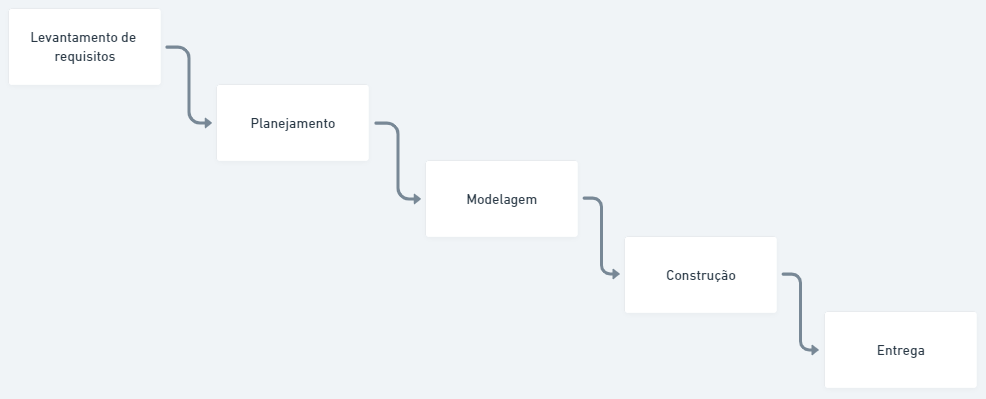
\includegraphics[width=1\textwidth]{./assets/figuras/ModeloCascata}}% measure width
	    \begin{minipage}{\wd0}
		    \usebox0
		    \caption{Fases do Modelo Cascata}
		    \label{fig:modelo-cascata}
		    \fonte{\citeonline{Pressman2015}}
	    \end{minipage}
    \end{figure}
    
    As fases podem  durar semanas ou meses e a fase seguinte só é iniciada após a fase anterior ter sido finalizada. Cada fase possui foco e atividades específicas:
        \begin{itemize}
            \item O projeto inicia com a fase de levantamento dos requisitos, na qual são realizadas atividades para identificação das necessidades do cliente do projeto;
            \item Em seguida ocorre a fase de planejamento, incluindo atividades de estimativas, cronograma e acompanhamento;
            \item O projeto avança pela fase de modelagem, na qual são realizadas a análise, o projeto do software e a construção de diagramas e modelos;
            \item Na sequência ocorre a fase de construção do software, a qual engloba as atividades de codificação e em seguida os testes do software;
            \item Por fim o projeto chega na fase final, na qual é realizada a entrega do software, é prestado suporte e são obtidos os \emph{feedbacks} do cliente.
            
        \end{itemize}
        
    As atividades de garantia de qualidade e de testes executadas na fase de construção se relacionam com o que é produzido nas fases anteriores. O modelo V (\autoref{fig:modelo-v})  é uma representação de quais atividades de teste estão relacionadas com os trabalhos de cada uma das fases do projeto. \cite{Pressman2015}
    
    \begin{figure}[!htb]
	    \centering
	    \sbox0{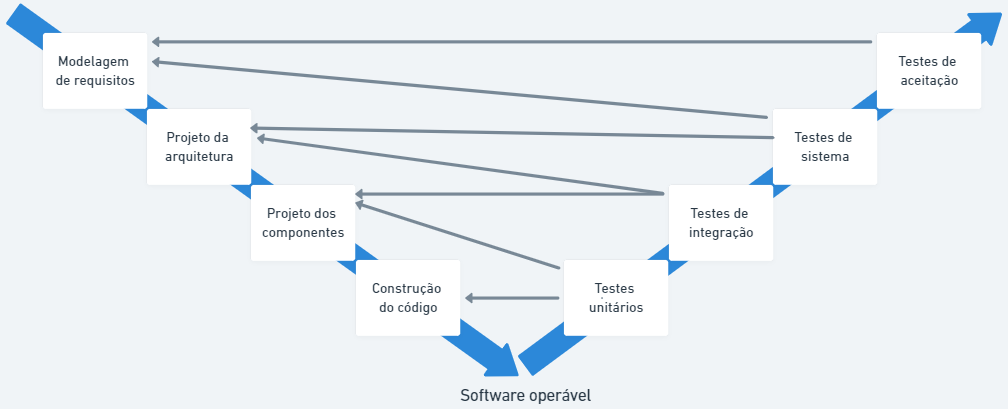
\includegraphics[width=1\textwidth]{./assets/figuras/ModeloV}}% measure width
	    \begin{minipage}{\wd0}
		    \usebox0
		    \caption{Modelo V}
		    \label{fig:modelo-v}
		    \fonte{\citeonline{Pressman2015}}
	    \end{minipage}
    \end{figure}
   
    As atividades de testes em processos sequenciais como o Cascata geralmente são realizadas manualmente por equipes dedicadas à execução de testes e ocorrem após finalizado o desenvolvimento do software. O software, que já está maduro o suficiente para ser executado, é utilizado nos testes de forma semelhante a que será utilizado pelos usuários finais, mas são informados dados de entrada específicos para teste. Os testes obtêm sucesso quando os comportamentos apresentados pelo software após a realização dos testes estiverem de acordo com aos comportamentos que são esperados que sejam apresentados, com base nas especificações produzidas nas fases anteriores e atendendo às necessidades dos usuários. 
    
    Como um dos objetivos das atividades de teste é o de revelar defeitos do software, a realização dos testes traz à tona erros cometidos em fases anteriores à de testes, como codificações incorretas, as quais causam falhas durante a execução ou comportamentos inconsistentes. Quanto mais tarde os defeitos forem encontrados, mais onerosa será a correção, pois além da correção do código do software para que não apresente mais tal defeito, poderá ser necessária a adequação da documentação produzida para que corresponda às alterações realizadas no software para corrigir o defeito.
    
    Testes de software tem relação direta com o processo de desenvolvimento de software, apresentando diversos conceitos e definições que serão exploradas no \autoref{chap:teste-de-software} com maior profundidade.
    
    O modelo cascata pode ser considerado o primeiro processo de desenvolvimento de software, mas ao longo dos anos sua eficácia passou a ser questionada. Alguns dos problemas encontrados são \cite{Pressman2015}:
        
        \begin{itemize}
            \item Os projetos reais raramente seguem um fluxo linear e sequencial, então as mudanças podem ocasionar confusão à medida que o projeto avança;
            \item Geralmente o cliente tem dificuldade de explicitar todas as suas necessidades no início do projeto, como é requerido pelo modelo cascata;
            \item As versões operáveis do software só estarão disponíveis próximos ao final do projeto, ocasionando em uma tardia detecção de erros e em descontentamentos do cliente.
        \end{itemize}
        
    Os processos sequenciais podem funcionar bem para projetos que possuem requisitos fixos e nos quais o projeto pode ser executado do começo ao fim de forma linear sem muitas mudanças, de maneira que são recomendados para projetos com incertezas ou mudanças frequentes o uso de processos ágeis.
    
    \section{PROCESSOS ÁGEIS}
    
    Devido aos problemas dos processos tradicionais, um grupo de profissionais se reuniu para propor uma alternativa ao processos sequenciais para desenvolvimento de software, defendendo que software é diferente de produtos tradicionais da Engenharia, portanto necessita de um processo de desenvolvimento diferente. Esse encontro resultou em um documento que é conhecido como manifesto ágil. Com o manifesto ágil passam a ser valorizados \cite{Valente2020}:
    \begin{itemize}
        \item Indivíduos e interações, mais do que processos e ferramentas;
        \item Validação do software mais do que uma documentação abrangente;
        \item Colaboração com o cliente mais do que negociação de contratos;
        \item Responder a mudanças mais do que seguir um plano.
    \end{itemize}
    
    O que caracteriza os processos ágeis são os ciclos de desenvolvimento iterativos e de curta duração, de uma a quatro semanas. O sistema é implementado gradualmente, começando pela implementação de uma versão com as funcionalidades que são mais prioritárias para o cliente. Após o cliente validar e aprovar essa versão, um novo ciclo, também chamado de iteração, é iniciado dando sequência ao desenvolvimento das demais funcionalidades também priorizadas pelo cliente, de maneira que todo ciclo produz uma versão funcional do software. O desenvolvimento é finalizado quando o cliente entende que todas as funcionalidades estão implementadas \cite{Valente2020}.
    
    Além dos valores do manifesto ágil, há 12 princípios de agilidade \cite{Pressman2015}:
    \begin{itemize}
        \item A maior prioridade é satisfazer o cliente através da entrega antecipada e contínua de software de valor;
        \item Mudanças nos requisitos são bem-vindas mesmo no fim do desenvolvimento, pois os processos ágeis aproveitam as mudanças como vantagem competitiva para o cliente;
        \item Deve-se entregar software funcionando frequentemente, de algumas semanas a alguns meses, preferindo-se os intervalos mais curtos;
        \item Pessoas de negócio e desenvolvedores devem trabalhar juntos diariamente ao longo do projeto;
        \item Deve-se construir projetos em torno de indivíduos motivados, dando a eles o ambiente e o suporte que precisarem, confiando neles para fazer o trabalho;
        \item O método mais eficiente e efetivo de transmitir informações com a equipe de desenvolvimento é a conversa cara a cara;
        \item Software funcionando é a principal medida de progresso;
        \item Processos ágeis promovem desenvolvimento sustentável. Os patrocinadores, desenvolvedores e usuários devem ser capaz de manter um ritmo constante indefinidamente;
        \item Atenção contínua para excelência técnica e bom projeto (\emph{design}) eleva a agilidade;
        \item Simplicidade, a arte da maximização do trabalho economizado, é essencial;
        \item As melhores arquiteturas, requisitos e projetos emergem de equipes auto-organizadas.
        \item Regularmente a equipe reflete sobre como se tornar mais efetiva, então sintoniza e ajusta seu comportamento de acordo.
    \end{itemize}
    
    Os processos que aplicam os valores e princípios do manifesto ágil mudam a visão sobre a responsabilidade pelas atividades de validação e testes. Todo time torna-se responsável por tais atividades e pela qualidade do software produzido, não sendo mais uma responsabilidade exclusiva de uma equipe de testes diferente da que realiza o desenvolvimento.
    
    Algumas outras características dos processos ágeis são: documentação apenas do que é essencial, sendo mais importante conseguir avançar mesmo com incertezas e possibilidade de mudança do que fazer um plano detalhado; não existência de uma fase dedicada ao projeto (\emph{design}), o qual também é feito de forma incremental; organização de times pequenos de desenvolvimento; e ênfase em novas práticas de desenvolvimento como programação em pares, testes automatizados e integração contínua. Devido a essas características, os processos ágeis são considerados leves, com pouca documentação. Essas características são genéricas e abrangentes, então foram criados métodos para auxiliar na adoção dos valores e princípios ágeis de forma concreta. \cite{Valente2020}. 
    
    Apesar de haver diversos métodos que aplicam os valores e princípios do manifesto ágil, neste trabalho será abordado o método intitulado Programação Extrema (\emph{Extreme Programming}), também conhecido como XP. O método XP é um dos mais bem definidos e completos e é o mais recomendado para entender a metodologia ágil, pois outros métodos ágeis empregam subconjuntos ou variações do XP, além de empregar práticas de testes automatizados em seu ciclo de vida \cite{Martin2020}, que são o foco deste trabalho.
        
        \subsection{Programação Extrema (XP)}
        
        O XP é um método leve recomendado para o desenvolvimento de software com requisitos imprecisos ou sujeitos a mudança e aplica as características dos processos ágeis. Entretanto o XP não define uma sequência detalhada de passos para produzir software, e sim um conjunto de valores e princípios que devem fazer parte da cultura e do dia a dia dos times de desenvolvimento, então esses valores e princípios são concretizados em práticas de desenvolvimento \cite{Valente2020}.
        
        O XP é conduzido pelos valores da comunicação, simplicidade, \emph{feedback}, coragem e respeito. Boa comunicação é essencial para evitar erros e também aprender com eles. A simplicidade é importante para focar em projetar mais as necessidades atuais que as futuras, produzindo projetos fáceis de serem implementados e que podem ser evoluídos futuramente, caso necessário. O rápido \emph{feedback} do cliente, dos membros da equipe e do próprio software através de uma estratégia de testes eficaz são essenciais para controlar riscos e diminuir prejuízos e retrabalhos. É necessário ter coragem e disciplina para projetar para as necessidades atuais, tendo em mente que as necessidades futuras podem mudar e exigir mudanças no projeto e no código. Os integrantes de time ágeis devem respeitar os demais membros da equipe, os demais envolvidos no projeto, o próprio software, além de ter respeito pelo processo XP \cite{Pressman2015}.
        
        A aplicação dos valores de simplicidade, comunicação e o \emph{feedback} representado pelos testes proporcionam um avanço mútuo, pois um valor beneficia o outro:  Os testes melhoram a comunicação através do registro das interfaces do programa; A comunicação melhora os testes aumentando as chances de defeitos serem revelados; A simplicidade é aumentada pelos testes, pois aumentam a possibilidade de refatorar código facilmente; E a simplicidade melhora os testes, pois um código mais simples é mais simples de se testar (\cite{beck1998}).
        
        Além desses valores, o XP também possui alguns princípios que são procedimentos mais concretos e pragmáticos \cite{Valente2020}:
        \begin{itemize}
            \item Humanidade: O principal recurso de uma empresa são seus colaboradores. Uma boa gestão de pessoas é a chave para o sucesso de projetos de software;
            \item Economicidade: Software é caro e quem está pagando por ele espera resultados econômicos e financeiros, então software não é uma obra de arte, mas uma produção que precisa de resultados econômicos;
            \item Benefícios Mútuos: As decisões tomadas nos projetos de software devem beneficiar a múltiplos envolvidos;
            \item Melhorias Contínuas: Como nenhum processo de desenvolvimento de software é perfeito, trabalhar em um software e em práticas de desenvolvimento que são aprimoradas a cada iteração a partir \emph{feedback} do cliente e da equipe é mais seguro;
            \item Falhas Acontecem: Software é uma das construções humanas mais complexas, então é esperado que softwares apresentem falhas e inconsistências. Elas não devem ser encobertas, mas também não devem ser usadas para punição do time;
            \item Passos de bebê (\emph{baby steps}): Pequenos progressos contínuos na direção certa são melhores que grandes revoluções, pois estas costumam gerar resultados negativos. Ou seja, é melhor concluir pequenas atividades constantemente que acumular uma grande quantidade de trabalho realizado aguardando ser concluído;
            \item Responsabilidade Pessoal: Os desenvolvedores devem ter clareza de seu papel e responsabilidade na equipe. O engenheiro de software que realiza a implementação também é responsável pelos testes e manutenção.
        \end{itemize}
        
        Além dos valores e princípios, o XP adota um conjunto de práticas para desenvolvimento ágil de software conhecidas como Ciclo de Vida. Muitas dessas práticas podem ser aplicadas inclusive em projetos que utilizam outros métodos ágeis. Algumas das práticas são orientadas para os negócios, outras para a equipe e outras são práticas técnicas (\autoref{fig:cicloXP}).
        
        \begin{figure}[!htb]
	        \centering
	        \sbox0{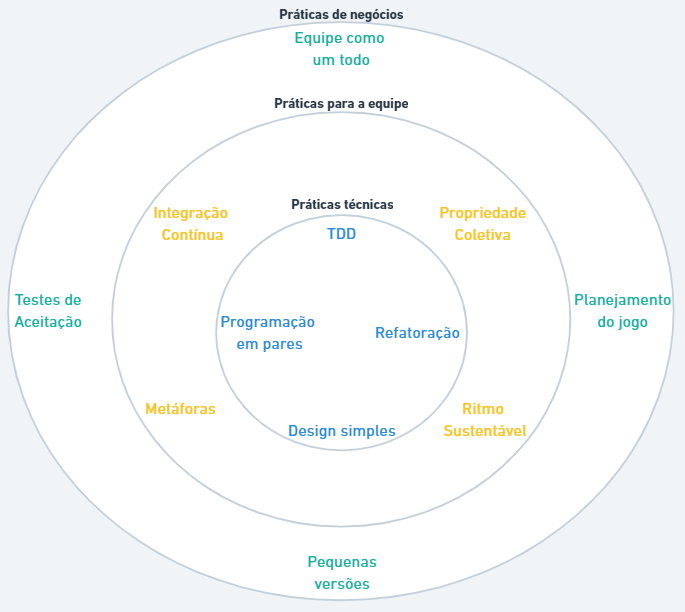
\includegraphics[width=1\textwidth]{./assets/figuras/CicloXP}}% measure width
	        \begin{minipage}{\wd0}
		        \usebox0
		        \caption{Ciclo de Vida XP}
		        \label{fig:cicloXP}
		        \fonte{\citeonline{Martin2020}}
	        \end{minipage}
        \end{figure}
        
            \subsubsection{Práticas orientadas para os negócios}
        
            As práticas orientadas para os negócios do XP definem como a equipe de desenvolvimento de software se comunica com os negócios e como o projeto é gerenciado \cite{Martin2020}:
            \begin{itemize}
                \item Planejamento do Jogo: Atividade que resulta na divisão do projeto em funcionalidades, histórias de usuário\footnote{É uma forma simples e leve de descrever requisitos de maneira concisa e sob a perspectiva do usuário.} e tarefas;
                \item Pequenas Versões: A equipe trabalha em pedaços pequenos do software;
                \item Testes de Aceitação: São testes realizados para verificar que o software está pronto e pode ser utilizado pelos usuários. Esses teste usam critérios de conclusão claros definidos para cada história ou tarefa individualmente, e também critérios válidos para todas as histórias ou tarefas desenvolvidas pelo time para determinar quando estão concluídas.
                \item Equipe como um todo: Uma equipe de desenvolvimento de software possui muitas atribuições e responsabilidades diferentes como codificação, testes e gerenciamento, todas convergindo para o mesmo objetivo.
            \end{itemize}
        
            \subsubsection{Práticas orientadas à equipe}
        
            As práticas orientadas à equipe determinam como a equipe de desenvolvimento se comunica e se gerencia \cite{Martin2020}:
            \begin{itemize}
                \item Ritmo Sustentável: Permite que o time desenvolva o projeto em um ritmo constante sem se esgotar no meio do projeto;
                \item Propriedade Coletiva: Evita que membros isolados da equipe detenham as informações do projeto apenas para si;
                \item Integração Contínua: o time de desenvolvimento constantemente deve integrar seu código a um repositório central. Feito isso, uma série de ações de construção (\emph{build}) da aplicação e de verificação, como a execução dos testes automatizados existentes, são realizadas de forma automática, oferecendo um \emph{feedback} rápido sobre o código integrado, permitindo identificar problemas rapidamente e mantendo a equipe ciente do andamento das atividades;
                \item Uso de Metáforas: Metáforas são utilizadas para que todos os envolvidos estabeleçam um vocabulário apropriado para o projeto e para que todos se entendam ao se comunicar sobre o software.
            \end{itemize}
        
            \subsubsection{Práticas técnicas}
        
            As práticas técnicas direcionam os programadores para atingirem a mais alta qualidade técnica\cite{Martin2020}:
            \begin{itemize}
                \item Programação em pares: Possibilita o compartilhamento de conhecimento entre a equipe, resultando em inovação e precisão;
                \item Projeto (\emph{design}) Simples: Garante que a equipe evite desperdiçar esforços;
                \item Refatoração: Proporciona a melhoria contínua e o aperfeiçoamento do que é produzido pela equipe;
                \item Desenvolvimento Guiado por Testes (\emph{Test Driven Development, TDD)}: Consiste em um conjunto de práticas por meio das quais, para cada pequena parte do software que será desenvolvida, os testes automatizados são implementados antes do código do software. Após criados, os testes são executados, porém falham inicialmente pois o código do software ainda não existe. Em seguida o desenvolvimento do código é iniciado e os testes são executados até que obtenham sucesso em sua execução. Por fim o código e os testes são evoluídos mantendo-se os testes alcançando sucesso em suas execuções.
            \end{itemize}
            
            A maioria das práticas do XP são utilizadas até mesmo por equipes que utilizam outro método ágil devido aos benefícios que essas práticas trouxeram para a produção ágil de software.


\chapter{TESTE DE SOFTWARE}
\label{chap:teste-de-software}

As atividades de teste de software estão presentes tanto nos processos tradicionais de desenvolvimento de software como nos processos ágeis, apesar das diferentes formas que as atividades são realizadas em cada um dos processos. Entretanto, em ambos os processos é necessário conhecimento dos fundamentos e técnicas de teste de software para que as atividades possam ser realizadas corretamente.

Para \citeonline{Myers2012}, testes de software são processos projetados para assegurar que códigos computacionais façam apenas o que propõem, não fazendo nada inesperado. Softwares devem ser previsíveis e consistentes, não apresentando surpresas para os usuários.

Segundo \citeonline{ISQTB2019}, o teste de software pode ter diferentes objetivos dependendo de fatores como: pontos de vista, níveis de teste, partes interessadas no teste, contextos dos componentes, softwares testados e ciclos de vida de desenvolvimento. Alguns desses objetivos são:

\begin{itemize}
    \item Avaliar produtos de trabalho;
    \item Verificar o cumprimento de requisitos especificados;
    \item Validar a completude de componentes ou softwares e sua conformidade com as expectativas dos usuários e outras partes interessadas;
    \item Gerar confiança no nível de qualidade de componentes ou softwares;
    \item Prevenir defeitos;
    \item Revelar falhas e defeitos;
    \item Prover informações para tomada de decisão;
    \item Reduzir o nível de risco de qualidade de software inadequada;
    \item Cumprir com requisitos e padrões regulatórios ou contratuais.
\end{itemize}

    \section{TESTES AUTOMATIZADOS}
    
    Testes automatizados são códigos computacionais que exercitam funcionalidades do software testado e verificam automaticamente os resultados obtidos. Essa abordagem traz algumas vantagens \cite{bernardo2008}:
    
    \begin{itemize}
        \item A rapidez e facilidade de executar os testes a qualquer momento, mesmo repetidas vezes;
        \item A reprodução do mesmo conjunto de ações em todas as execuções, permitindo simular precisamente todos os passos que geram comportamentos específicos, evitando falhas humanas e contribuindo para a identificação de comportamentos indesejados;
        \item A possibilidade de executar diferentes testes simultaneamente;
        \item A possibilidade de realizar testes em condições em que há dificuldade de realizá-los manualmente, como situações elaboradas e complexas envolvendo combinações de comandos e operações, ou então a simulação de utilizações simultâneas do software ou da parte dele que está sendo testada.
    \end{itemize}

    \citeonline{sommerville2019} descreve que os métodos de teste automatizados são compostos por três partes:

    \begin{itemize}
        \item Configuração: o software a ser testado é iniciado com as entradas e saídas esperadas. Por exemplo, são instanciados e inicializados os objetos que pretende-se testar.
        \item Chamada: são realizadas as chamadas aos métodos ou objetos que estão sendo testados.
        \item Asserção: é realizada a comparação dos resultados obtidos nas chamadas com os resultados esperados, sendo a asserção verdadeira quando os resultados obtidos e esperados são iguais. Os testes obtêm sucesso quando a asserção é verdadeira e falham quando a asserção é falsa.
    \end{itemize}


    \section{NÍVEIS DE TESTE}
    \label{section:niveis-de-teste}

    Para \citeonline{Pressman2015}, uma estratégia na qual os testes são realizados apenas após o sistema estar finalizado não funciona e resulta em um software com defeitos. Uma abordagem preferencial é seguir uma estratégia que emprega testes de forma incremental, começando por testes de unidades individuais do software, seguido por testes de integração de unidades e finalizando com testes utilizando o sistema completo. \citeonline{ISQTB2019} nomeia essas diferentes instâncias do processo de testes como níveis de teste.

        \subsection{Teste unitário}
        
        Teste unitário, também conhecido como teste de unidade ou teste de componente, tem foco na verificação da menor unidade do software, como um componente ou um módulo de software, e tem enfoque na lógica interna de processamento e nas estruturas de dados dos componentes \cite{Pressman2015}. A complexidade dos testes e os erros revelados por eles são restritos ao escopo do teste unitário. Esse teste pode ser realizado em paralelo para vários componentes.

        Para \citeonline{sommerville2019}, os testes unitários devem ser automatizados sempre que houver a possibilidade. Segundo \citeonline{Valente2020}, os testes unitários são aplicados de forma automatizada a pequenas unidades do código, normalmente classes, e são isolados do restante do software.

        Os testes unitários não dependem que todo o software esteja finalizado para serem realizados e obterem sucesso, basta que o componente testado tenha sido implementado. O componente testado, entretanto, pode ter dependência de outros componentes ainda não implementados, o que pode tornar o processo de testes mais lento \cite{sommerville2019}. Por exemplo, componentes que realizam comunicação com banco de dados podem precisar de uma etapa prévia de configuração para que o banco possa ser utilizado, podendo atrasar a realização dos testes.
        
        Os testes unitários trazem algumas vantagens para o desenvolvimento do software \cite{Valente2020}:
        
        \begin{itemize}
            \item Revelar defeitos ainda durante o desenvolvimento do software em uma fase em que as correções são menos custosas, evitando que os defeitos cheguem até o usuário final;
            \item Adicionam proteção contra defeitos causados por modificações no código, pois se um defeito for introduzido, os testes que exercitam a parte do software afetada pelo defeito deixarão de obter sucesso;
            \item Auxiliam na documentação e especificação do código, pois revelam detalhes do comportamentos do código testado.
        \end{itemize}

        Como o teste unitário foca nas partes internas do componente testado e em sua verificação de forma isolada, podem ser utilizados objetos simulados (\emph{mock objects}) no lugar das dependências do componente testado. Esses objetos simulam a funcionalidade e possuem a mesma interface do componente testado \cite{sommerville2019}. Por exemplo, é possível utilizar um objeto simulando um banco de dados com poucos itens que podem ser acessados rapidamente, eliminando a sobrecarga de utilizar um banco de dados real. Também é possível utilizar objetos para simular a ocorrência de operações anormais ou que não ocorrem com frequência.
        
        Para que os testes unitários atinjam seus objetivos eles devem atender a algumas propriedades. Os testes devem ser rápidos, independentes, determinísticos,  auto-verificáveis e escritos a tempo. Essas propriedades são conhecidas como princípios FIRST, acrônimo formado pelas iniciais das palavras em inglês referentes a cada um dos princípios  (\emph{fast, independent, repeatable, self-checking} e \emph{timely}).  
        
        \cite{Valente2020} descreve cada um desses princípios como:
        
        \begin{itemize}
            \item Rápidos (\emph{fast}): os testes unitários devem executar rapidamente, ou seja, em um tempo de execução de alguns milissegundos, pois serão executados frequentemente e devem fornecer \emph{feedback} rápido sobre o funcionamento do código. Testes que não possam ser executados rapidamente podem ser separados em um conjunto de testes que têm maior tempo de execução e que serão executados com menor frequência;
            \item Independentes (\emph{independent}): o resultado da execução de cada teste não deve ser afetado pela ordem de execução dos mesmos, podendo até mesmo serem executados de forma paralela, ou seja, os testes não devem depender de ações realizadas por outros testes;
            \item Determinísticos (\emph{repeatable}): Os testes devem ter o mesmo resultado todas as vezes que executados nas mesmas condições, ou seja, apenas alterações no código devem ser capazes de alterar o resultado dos testes. Testes com resultados não determinísticos são chamados de testes erráticos (\emph{flaky});
            \item Auto-verificáveis (\emph{Self-checking}): Os resultados de execução dos testes devem ser verificados com facilidade, sendo autoexplicativos e não dependendo de ações manuais para que sejam interpretados. Os resultados devem mostrar claramente quais testes obtiveram sucesso e quais falharam, e caso o teste falhe, devem possibilitar identificar rapidamente as asserções falsas;
            \item Feitos a tempo (\emph{timely}): Os testes devem ser escritos o quanto antes, se possível até mesmo antes do código que será testado, como é feito no desenvolvimento guiado por testes.
        \end{itemize}
        
        Além dos princípios adotados para que os testes sejam efetivos, algumas características, chamadas de \emph{test smells}, devem ser evitadas sempre que possível \cite{Valente2020}. Por exemplo:
        \begin{itemize}
            \item Testes obscuros, compreendidos por testes longos, complexos e difíceis de entender. O ideal é testar apenas um requisito de sistema em cada teste;
            \item Uso de estruturas condicionais e laços de repetição no código de teste;
            \item Duplicação de código em testes.
        \end{itemize}

        \subsection{Testes de integração}

        Teste de integração, também chamado de teste de serviço, verifica a integração entre diferentes componentes do software ou entre diferentes sistemas. Para \citeonline{Valente2020}, o teste de integração executa serviços ou funcionalidades completas, engloba um maior número de componentes do software do que os testes unitários e não utiliza objetos simulados, sendo um teste maior, mais demorado e, portanto, executado com menos frequência que o teste unitário.

        \subsection{Testes de sistema}
        
        Testes de sistema, também chamados de testes de ponta a ponta ou testes de interface, são testes que manipulam todos os componentes e dependências do software de forma integrada. Esses testes simulam o uso real do sistema e são os testes que necessitam de maior esforço para serem implementados, que têm uma maior dificuldade para serem escritos e que levam mais tempo para serem executados. \cite{Valente2020}.

    \section{TIPOS DE TESTE}
    
    Testes de software podem ser categorizados de acordo com os diferentes objetivos, os quais são relacionados às diferentes características do software testado. Os diferentes tipos de teste podem ser aplicados nos diferentes níveis de teste.
        
        \subsection{Testes funcionais}
        \label{section:testes-funcionais}
        
        Os testes funcionais verificam os requisitos funcionais do sistema ou componente testado, ou seja, o que o software deve ser capaz de fazer, as ações e funcionalidades que deve ser capaz de operar. Os testes podem se basear nas documentações criadas para especificar os requisitos funcionais, mas também podem se basear em requisitos funcionais não documentados, que nesse caso são revelados por necessidades do processo do negócio ou pela comparação do software testado com softwares com propósito semelhante. Esses testes devem ser realizados em todos os níveis de teste, podendo ter diferentes focos em cada nível. A porcentagem de requisitos funcionais que são exercitados pelos testes é uma forma de medir a eficácia dos testes funcionais, medida que é chamada de cobertura funcional \cite{ISQTB2019}.
        
        \subsection{Testes não funcionais}
        \label{section:testes-nao-funcionais}
        
        Testes não funcionais têm o objetivo de verificar requisitos não funcionais do software testado, ou seja, as características do software que não estão relacionadas às funcionalidades, mas a quão bem o software ou componente testado se comporta e se ele possui as características que são esperadas que possua, mas focando em questões como desempenho, escalabilidade, usabilidade e outras características que não são requisitos funcionais
        
        Testes não funcionais verificam as características de qualidade ou os atributos não funcionais do software ou componente e utilizam critérios que podem ser medidos, como por exemplo, o tempo de resposta \cite{ISQTB2019}.
        
         \subsection{Testes de confirmação}
        Após corrigir um defeito no software é necessário exercitar novamente o software reproduzindo as ações que revelaram o defeito.
        
        O teste de confirmação verifica se as correções realizadas no software realmente corrigiram com sucesso os defeitos que pretendiam corrigir. O software pode ser testado realizando-se novamente os testes que falharam devido ao defeito, além de novos testes que podem ser identificados a partir da correção implementada. O teste de confirmação é realizado em todos os níveis de teste. \cite{ISQTB2019}
        
        \subsection{Testes de Regressão}
        
       Após modificar o código de um software, seja para correções em funcionalidades ou em partes do software já em funcionamento ou para adição de novas funcionalidades ao software, é comum que aconteçam erros de regressão, ou seja, defeitos que foram inseridos em partes do software que anteriormente funcionavam corretamente.
       
       Testes de regressão têm o objetivo de detectar os comportamentos indesejados que podem ter sido inseridos acidentalmente em qualquer parte do software pelas modificações realizadas no código, sendo muito importante a realização de testes de regressão especialmente em ciclos de vida de desenvolvimento iterativo e incremental, nos quais há frequente alteração no código. Como os conjuntos de teste de regressão são executados com frequência e geralmente evoluem lentamente, são fortes candidatos à automação, que deve começar já no início do projeto, e assim como os testes de confirmação, os testes de regressão são realizados em todos os níveis de teste. \cite{ISQTB2019}.
       
       O teste de regressão pode ser realizado através da execução de todo o conjunto de testes criados para o software ou parte desse conjunto.

    \section{TÉCNICAS DE TESTE}
    
    As técnicas de teste são formas sistemáticas de identificar quais testes devem ser executados, suas condições e os dados que devem ser utilizados nos testes.
    
        \subsection{Teste caixa-branca}
        
        As técnicas de teste de caixa-branca baseiam-se em análises da estrutura interna do software ou componente testado para identificar os testes necessários, concentrando-se na estrutura e processamento. Podem ser aplicados em todos os níveis de teste, mas são mais utilizados em testes unitários e de integração. Os testes de caixa-branca são frequentemente usados como forma de medir a eficácia dos testes através da cobertura de um conjunto de elementos estruturais, ou seja, a quantidade desses elementos que está sendo exercitada durante a execução dos testes. No nível de testes unitários há ferramentas que medem a cobertura do código calculando a porcentagem de elementos executáveis que foram exercitados pelo conjunto de testes executados \cite{ISQTB2019}.
    
        \subsection{Teste caixa-preta}
        
        As técnicas de teste de caixa-preta baseiam-se na análise das especificações do software e dos requisitos para identificar os testes necessários, incluindo testes funcionais e não funcionais. Concentram-se na identificação das condições e dados de testes adequados e no que deve ser retornado pelo software ou componente testado, mas sem envolver a análise das estruturas internas do software, \cite{ISQTB2019}.
    